\section{Introduction}
\label{introduction}

Here we are interested in autonomous driving systems. In the simplest scenario, this can be thought as a cognitive driving intelligence layered on top of a basic vehicle platform

Basic vehicles already run a larg amount of software. In many cases, this software gas to meet tight constraints with respect to real time processing,
failure rate, maintainability and safety \cite{Serban}. Adding cognitive intelligence into the mix leads to new software components deployed on existing platforms.
Thus, a clear mapping between functional goals and software componenents is needed. 

Software architecture has been introduced  as a means to manage complexity in software systems and help assess functional and non-functional attributes before the 
build phase. A good architecture is known to help ensure tat a system satisfies key requirements in areas such as functional suitability, performance,
reliability or interoperability \cite{Garlan2000}. 


\begin{framed}
\theoremstyle{remark}
\begin{remark}{\textbf{Functional Architecture}}

A functional architecture refers to a logical decomposition of the system into component and subcomponents as well as data flows between them.  
This decomposition is done without reference to the actual technical implementation of the architectural elements in terms of hardware and/or software.

Furtheremore, the term is used analogously to the term {\em functional concept} described in the ISO 26262 automotive standard; a specification
of intended functions and necessary interactions in order to achieve desire behaviors. Functional architecture design corresponds to the second
step in the V-model. This software development life cycle is imposed by the mandatory compliance with the ISO 26262 automotive standard.

\end{remark}
\end{framed}



\section{Functional Components}

A common segregation of the principal functional architectural components of an autonomous driving systems consists of the following modules \cite{Bahere}:

\begin{itemize}
\item Perception
\item Decision and Control
\item Vehicle platform manipulation
\end{itemize}


The Perception component is responsible for perceiving the external environment/context in which the vehicle operates.  
The Decision and Control component handles the control of the vehicle motion in response to the external environment that is perceived. 
The Vehicle platform manipulation deals mostly with sensing and actuation of the vehicle with the intension of achieving a desired motion \cite{Bahere}.
Each of the aforementioned functional modules has several components which is shown schematically in figure \ref{autonomous_driving_components}. 



\begin{figure}[!htb]
\begin{center}
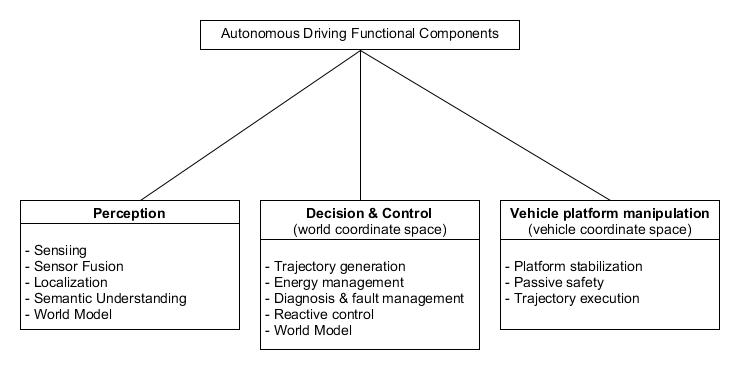
\includegraphics[scale=0.380]{img/autonomous_driving_components.jpg}
\end{center}
\caption{Autonomous driving functional components.}
\label{autonomous_driving_components}
\end{figure}


\section{Perception}

Sensing means gathering data on physical variables using sensors. Perception refers to the semantics 
i.e. interpretation and understanding, of the data in terms of high level concepts relevant to the task in hand.

The sensing components can be categorized into \cite{Bahere}
\begin{itemize}
\item Those sensing the state of the vehicle 
\item Those sensing the state of the environment in which the vehicle operates
\end{itemize}
Another categorization of sensor components is from the viewpoint of systems integration. 
This categorization depends on the amount of processing needed to extract relevant information from the sensor data.

\subsection{Sensor Fusion}

The component considers multiple sources of information to construct a hypothesis about the state of the environment. 
Additionally, the component establishes confidence values for state variables. 
The component may also perform object association and tracking. Association refers to correlating pieces of
information from multiple sensors to conclude that they refer to one and the same object.

For certain system configurations the sensor fusion block may also be used to eliminate some un-associated objects and data that 
is strongly likely to be superfluous or noise. This reduces the computation and communication load on 
subsequent components like the decision and control which need to work with the perceived data.


\subsection{Localization}

The localization component is responsible for determining the location of the vehicle with respect to a global map with needed accuracy.
Further, it may also aid the sensor fusion component to perform a task known as map matching wherein physical location s of detected objects are referenced to map’s coordinate system. 

The component typically uses sensors like GPS and inertial measurement units (IMU).

Certain algorithms try to improve on the accuracy of localization by identifying visual landmarks via cameras. The base map layers have traditionally been stored on board however tiled maps can also be used. In the latter case tiles can be dynamically streamed from a service provider based on the vehicle location and may be locally cached.

\subsection{Semantic Understanding}
This component may include classifiers for detected objects and it may annotate the objects with references to physical models that predict possible future behavior. Detection of ground planes, road geometries, representation of driveable areas may also happen in this component.

In some cases, the semantic component may also use the ego vehicle data to continuously parametrize a model of the ego vehicle for purposes of motion control, error detection and potential degradation of functionality.

\subsection{World Model}
This component holds the state of the external environment as perceived by the ego vehicle.

A world model component can be characterized as either passive or active \cite{Bahere}. 
The former is more like a data store and may lack semantic understanding of the stored data. 
Hence, by itself it cannot perform physics related computations on the data it holds. 
Therefore, it cannot actively predict the state of the world given specific inputs. 
The active world model may incorporate kinematic and dynamic models of the objects it contains 
and be able to evolve beliefs of the world states when it is given a sequence of inputs \cite{Bahere}.

Other components (like Decision and Control) my request a set of predictions of future world states for a specific set of
inputs in order to determine the optimal inputs to be applied.
Despite its inability to actively make calculations based on the data it contains, the passive world model is perhaps the most commonly found approach in autonomous driving projects \cite{Bahere}. 




\subsubsection{Local Dynamic Maps}

The Local Dynamic Maps (LDM) is an approach to model a passive world model \cite{Bahere, ETSITR102}. 
An LDM is implemented as a database but conceptually it can be understood as a layered map. 

\begin{figure}[!htb]
\begin{center}
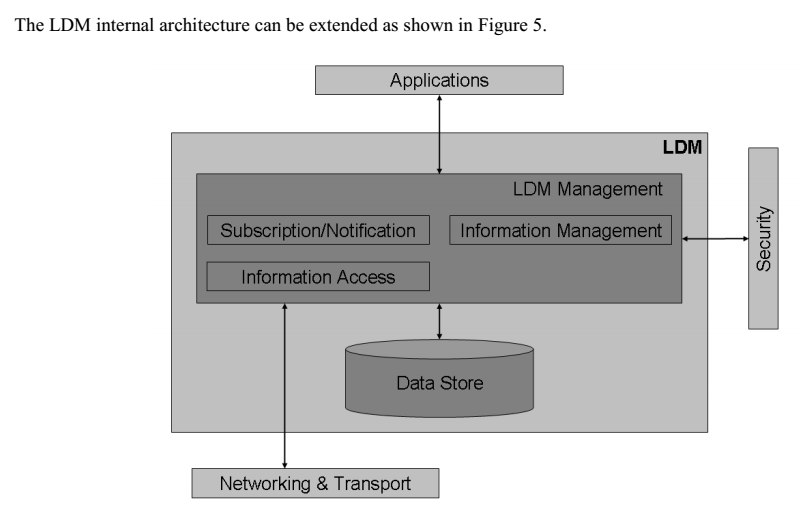
\includegraphics[scale=0.380]{img/ldm_internal_architectuer.png}
\end{center}
\caption{LDM internal architecture.}
\label{ldm_internal_architectuer}
\end{figure}

The bottom most layers represent the most static beliefs about the world while the topmost layers represent the most dynamic in the sense of time. For example, the lowermost layer may be populated with a static map of the immediate surroundings of the vehicle (roads, permanent features etc.). The next layer may contain temporary objects
like diversions due to construction work. The final layer would be populated by fast moving objects detected by the rest of the perception system (other vehicles, pedestrians etc.)\cite{ETSITR102}. 

Regardless of its implementation, the world model typically provides an interface to query its contents, add or remove data, concurrency, access control, replication over distributed computational media etc. It may also hold historical information about some or all of its contents.  


\section{Decision \& Control}
The functional components in this category are concerned with the vehicle behavior 
in the context of the external environment it is operating in \cite{Bahere}. Typically, modules in this category refer to the vehicle as a whole and the way it
moves in its environment. Furthermore, energy, fault management concerns and reactive control to unexpected events in the environment are also handled. 

\subsection{Trajectory Generation}
The component continuously generates obstacle free trajectories in the world coordinate system. The trajectory generation is constrained by factors such as energy availability, limitations of the vehicle platform (e.g. non-holonomicity), faults and failures. 

\subsection{Energy Management}

\subsection{Diagnosis and fault Management}

\subsection{Reactive Control}
These components are used for immediate responses to unanticipated stimuli from the environment. Existing vehicle features like collision mitigation  by braking may be considered as reactive control. These components execute in parallel with the nominal system, and if a threat is identified, their output overrides the nominal behavior requests. Their SENSE-PLAN-ACT loops typically run at least an order of magnitude faster than the  nominal system loop \cite{Bahere}.

It is sometimes the case that what is considered reactive behavior in the presence of unexpected events, can be dealt with by very fast deliberative behavior. As an example consider the Autonomous Emergency Breaking (AEB) that some passenger cars feature. This is considered a reactive function that monitors a small subset of sensors
(compared to full autonomous driving) and initiates braking action in case of imminent collision with a moving or stationary obstacle. The function is constantly active, when it is enabled, and may generate a deceleration demand that overrides other demands on the propulsion subsystem. However, if the perception and trajectory generation components are sufficiently fast, they could detect the threat and generate appropriate trajectories as part of their normal operation and thus negating the need for a specialized AEB system \cite{Bahere}.  

\section{Vehicle Platform Manipulation}

This category groups the components that are directly responsible for the motion of the vehicle. They abstract the principal actuation systems and also
provide minimum level of stability to the platform while it is in motion. 

Although not directly related to propulsion, components related to passive vehicle safety may be included in this category, since they are closely related to scenarios arising from undesirable propulsion and may be triggered by the decision and control components.

\subsection{Platform Stabilization}

Usually components in this category are related to traction control, electronic stability and anti-lock braking features. The task of these components is to keep the vehicle platform in a controllable state during operation. Unreasonable motion requests may be rejected or adapted to stay within the physical capabilities and safety envelope of the vehicle.

\subsection{Trajectory Execution}

These components are responsible for executing the trajectory generated by the Decision and Control modules. This is achieved by a combination of longitudinal acceleration (propulsion), lateral acceleration  (steering) and deceleration (braking). Since most vehicles already incorporate such components, these can be considered as traditional from the perspective of autonomous driving development.


\section{Functional Distribution}

We can consider an autonomous vehicle as comprising of two layers; a cognitive 
layer responsible for intelligently operating the vehicle and the vehicle platform which from the outside it corresponds to the vehicle chassis. 

Naturally, this separation leads to the following two questions:

\begin{itemize}
\item What kind of information should flow between the cognitive and the vehicle platform layers?
\item What changes are necessary if the vehicle platform is to be controlled by a machine and not a human being?
\end{itemize}

The answers to the previous questions depend on the distribution of functionality attributed to each layer. Currently, most autonomous vehicles are built on top of existing production vehicles therefore the pattern followed is: The vehicle platform
contains a network of ECUs that control the functionality such as longitudinal and lateral dynamics or breaking. The manufacturer then allows for some sort of gateway that in return allow for a limited number of set points to be transmitted to the vehicle ECUs.  As an example, the cognitive driving intelligence may continuously regulate the set-point of the cruise control function in the vehicle.

From a theoretical perspective, the functionality  between the driving intelligence and the vehicle platform can be allocated such that it lies between two extreme cases. The one extreme is when the cognitive agent directly controls the torque outputs of the vehicle platform actuators using a distributed I/O approach. In this case the cognitive agent needs an intimate familiarity with the vehicle platform. Thus, this extreme implies a possibly large degree of coupling between the two layers. The other extreme, Figure 2 (b), treats both the cognitive
driving intelligence as well as the vehicle platform as two cooperating, relatively autonomous entities. Neither knows the intimate details about the other. The driving agent  makes motion demands of the vehicle platform in world coordinates, which the latter makes a best effort to fulfill. The task of the driving intelligence is to perceive the world and make motion requests in this world, while
the task of the vehicle platform is to realize the desired motion requests while keeping its own features and limitations in mind. In such an ideal de-coupling, the same driving intelligence should be able to operate a variety of vehicle platforms, provided the acceleration interface remains the
same.   

We have already mentioned that the first architecture, introduces strong coupling between the two layers. Furthermore, in order to perform closed loop propulsion control of the vehicle platform, the driving intelligence would need a fairly detailed model of the platform, including its dynamics and the constraints on the vehicle actuators and sensors. Performing fine-grained (low time horizon) control of the actuators by using motion feedback from the perception system places unreasonably high demands on the technical implementation and performance of the perception system. On the other hand, the latter architecture is attractive because it enables a relatively clean separation of concerns. The driving intelligence need not be concerned with the finer details of
how the motion it desires is achieved. The vehicle platform need not be concerned with how and why the motion commands are generated - only whether they are realizable and if so, how to best realize them given the current platform capabilities. Concepts related to stabilization of the platform,
like traction control, anti-lock brakes etc. are transparently realized by the vehicle platform, without the driving intelligence having to be aware of them.

Following the best practices of separating concerns and loose couplings, one should strive to  achieve as clean a split as possible, between the driving intelligence and vehicle platform. This lowers the cognitive complexity (cognitive effort needed to understand a model) of the architecture, as well
as reduces the potential for feature interaction and other undesirable emergent behavior. It also enables better reuse of the driving intelligence and vehicle platform in other projects. That said, any assumptions made regarding the behavior and performance of the vehicle platform need to
be made explicit. This is especially true for end-to-end latencies on the fulfillment of acceleration requests, and interpretation of sensor data by the controllers in the vehicle platform. The approach (of Figure 2 (b)) places high demands
on the functionality available in the vehicle platform, with regards to its abilities for keeping the platform stable, and retaining basic self-protection measures which may include reactive control. In practice, this is unlikely to be an issue because the high-end vehicles of most automotive OEMs today already incorporate such functionality and it is these high-end vehicles that are the most likely candidates for receiving upgrades to self-driving functionality. The principal modifications needed to these vehicles, as self-driving vehicle platforms, would be in the area of sub-system redundancy,
to increase the platform reliability and safety.


\section{Functional Architecture (An example)}

As shown in Figure 3, the sensing and world model components, although conceptually unified, are split into those dealing with the external environment of the vehicle, and
those dealing with the Ego vehicle platform. The split helps to achieve separate technical implementations, if required, when the functional architecture is eventually refined to a
technical architecture, following the ISO26262 process. The inter-component arrows in Figure 3 represent data-flows in
the direction of the arrow. As shown, the outputs of the sensing components go to the rest of the perception and decision and control components, either directly or indirectly, depending on the level of processing and fusion that is needed.

In our experience, it is useful to establish a data link between localization and sensor fusion. Certain sensors may exhibit repeatable tendencies at fixed locations along specific routes, like increase in false positives, dropouts etc. Changing the level of confidence in a sensor, based on geographical
location is an interesting line of research and the architecture should not be a limiting factor.
Another interesting data link in Figure 3 is the connection from the semantic understanding component to the sensor components. This is useful in at least three scenarios:

\begin{itemize}
\item  Firstly, some specialized autonomous driving situations benefit from so-called focused attention mechanisms. Focused
attention means exploring a specific part of the environment more deeply. This may require physical motion of the sensors and/or configuration changes to the sensors (panning a
camera to a different field of view, changing the ’zoom’ of a lens, etc.). Today, most sensors of most autonomous vehicles are physically fixed to a constant pose with respect to the vehicle coordinate system. But in the domain of mobile
and cognitive robotics, it is quite common to have, for example, a pan-tilt-zoom camera to aid the robot in a search task. 
\item  Secondly, calibration changes to the sensors may be needed at runtime (e.g. changing exposures based on time of day, triggering re-calibration if changes in physical alignment are suspected). 
\item Thirdly, if communication transceivers are considered as a kind of sensor/actuator, the semantic understanding component can use it to respond to incoming communication requests, publish ego vehicle information and make asynchronous requests for information. Such communication requirements are often an integral part of scenarios like cooperative driving, where a vehicle maintains constant communication to the infrastructure and other vehicles in the vicinity.
\end{itemize}






